\documentclass[twoside]{book}

% Packages required by doxygen
\usepackage{fixltx2e}
\usepackage{calc}
\usepackage{doxygen}
\usepackage{graphicx}
\usepackage[utf8]{inputenc}
\usepackage{makeidx}
\usepackage{multicol}
\usepackage{multirow}
\PassOptionsToPackage{warn}{textcomp}
\usepackage{textcomp}
\usepackage[nointegrals]{wasysym}
\usepackage[table]{xcolor}

% Font selection
\usepackage[T1]{fontenc}
\usepackage{mathptmx}
\usepackage[scaled=.90]{helvet}
\usepackage{courier}
\usepackage{amssymb}
\usepackage{sectsty}
\renewcommand{\familydefault}{\sfdefault}
\allsectionsfont{%
  \fontseries{bc}\selectfont%
  \color{darkgray}%
}
\renewcommand{\DoxyLabelFont}{%
  \fontseries{bc}\selectfont%
  \color{darkgray}%
}
\newcommand{\+}{\discretionary{\mbox{\scriptsize$\hookleftarrow$}}{}{}}

% Page & text layout
\usepackage{geometry}
\geometry{%
  a4paper,%
  top=2.5cm,%
  bottom=2.5cm,%
  left=2.5cm,%
  right=2.5cm%
}
\tolerance=750
\hfuzz=15pt
\hbadness=750
\setlength{\emergencystretch}{15pt}
\setlength{\parindent}{0cm}
\setlength{\parskip}{0.2cm}
\makeatletter
\renewcommand{\paragraph}{%
  \@startsection{paragraph}{4}{0ex}{-1.0ex}{1.0ex}{%
    \normalfont\normalsize\bfseries\SS@parafont%
  }%
}
\renewcommand{\subparagraph}{%
  \@startsection{subparagraph}{5}{0ex}{-1.0ex}{1.0ex}{%
    \normalfont\normalsize\bfseries\SS@subparafont%
  }%
}
\makeatother

% Headers & footers
\usepackage{fancyhdr}
\pagestyle{fancyplain}
\fancyhead[LE]{\fancyplain{}{\bfseries\thepage}}
\fancyhead[CE]{\fancyplain{}{}}
\fancyhead[RE]{\fancyplain{}{\bfseries\leftmark}}
\fancyhead[LO]{\fancyplain{}{\bfseries\rightmark}}
\fancyhead[CO]{\fancyplain{}{}}
\fancyhead[RO]{\fancyplain{}{\bfseries\thepage}}
\fancyfoot[LE]{\fancyplain{}{}}
\fancyfoot[CE]{\fancyplain{}{}}
\fancyfoot[RE]{\fancyplain{}{\bfseries\scriptsize Generated on Mon Jan 12 2015 20\+:10\+:03 for “\+Traffic\+Simulator“ by Doxygen }}
\fancyfoot[LO]{\fancyplain{}{\bfseries\scriptsize Generated on Mon Jan 12 2015 20\+:10\+:03 for “\+Traffic\+Simulator“ by Doxygen }}
\fancyfoot[CO]{\fancyplain{}{}}
\fancyfoot[RO]{\fancyplain{}{}}
\renewcommand{\footrulewidth}{0.4pt}
\renewcommand{\chaptermark}[1]{%
  \markboth{#1}{}%
}
\renewcommand{\sectionmark}[1]{%
  \markright{\thesection\ #1}%
}

% Indices & bibliography
\usepackage{natbib}
\usepackage[titles]{tocloft}
\setcounter{tocdepth}{3}
\setcounter{secnumdepth}{5}
\makeindex

% Hyperlinks (required, but should be loaded last)
\usepackage{ifpdf}
\ifpdf
  \usepackage[pdftex,pagebackref=true]{hyperref}
\else
  \usepackage[ps2pdf,pagebackref=true]{hyperref}
\fi
\hypersetup{%
  colorlinks=true,%
  linkcolor=blue,%
  citecolor=blue,%
  unicode%
}

% Custom commands
\newcommand{\clearemptydoublepage}{%
  \newpage{\pagestyle{empty}\cleardoublepage}%
}


%===== C O N T E N T S =====

\begin{document}

% Titlepage & ToC
\hypersetup{pageanchor=false,
             bookmarks=true,
             bookmarksnumbered=true,
             pdfencoding=unicode
            }
\pagenumbering{roman}
\begin{titlepage}
\vspace*{7cm}
\begin{center}%
{\Large “\+Traffic\+Simulator“ \\[1ex]\large 1.\+0 }\\
\vspace*{1cm}
{\large Generated by Doxygen 1.8.8}\\
\vspace*{0.5cm}
{\small Mon Jan 12 2015 20:10:03}\\
\end{center}
\end{titlepage}
\clearemptydoublepage
\tableofcontents
\clearemptydoublepage
\pagenumbering{arabic}
\hypersetup{pageanchor=true}

%--- Begin generated contents ---
\chapter{Hierarchical Index}
\section{Class Hierarchy}
This inheritance list is sorted roughly, but not completely, alphabetically\+:\begin{DoxyCompactList}
\item \contentsline{section}{Car\+Position}{\pageref{class_car_position}}{}
\item Cloneable\begin{DoxyCompactList}
\item \contentsline{section}{Car}{\pageref{class_car}}{}
\begin{DoxyCompactList}
\item \contentsline{section}{Taxi}{\pageref{class_taxi}}{}
\end{DoxyCompactList}
\end{DoxyCompactList}
\item \contentsline{section}{Lane}{\pageref{class_lane}}{}
\item \contentsline{section}{Light}{\pageref{class_light}}{}
\item Runtime\+Exception\begin{DoxyCompactList}
\item \contentsline{section}{Overflow\+Exception}{\pageref{class_overflow_exception}}{}
\end{DoxyCompactList}
\item \contentsline{section}{Simulation}{\pageref{class_simulation}}{}
\item \contentsline{section}{Traffic\+System}{\pageref{class_traffic_system}}{}
\end{DoxyCompactList}

\chapter{Class Index}
\section{Class List}
Here are the classes, structs, unions and interfaces with brief descriptions\+:\begin{DoxyCompactList}
\item\contentsline{section}{\hyperlink{class_car}{Car} \\*The Class \hyperlink{class_car}{Car} }{\pageref{class_car}}{}
\item\contentsline{section}{\hyperlink{class_car_position}{Car\+Position} \\*The Class \hyperlink{class_car_position}{Car\+Position} }{\pageref{class_car_position}}{}
\item\contentsline{section}{\hyperlink{class_lane}{Lane} \\*The Class \hyperlink{class_lane}{Lane} }{\pageref{class_lane}}{}
\item\contentsline{section}{\hyperlink{class_light}{Light} \\*The Class \hyperlink{class_light}{Light} }{\pageref{class_light}}{}
\item\contentsline{section}{\hyperlink{class_overflow_exception}{Overflow\+Exception} \\*The Class \hyperlink{class_overflow_exception}{Overflow\+Exception} }{\pageref{class_overflow_exception}}{}
\item\contentsline{section}{\hyperlink{class_simulation}{Simulation} \\*The Class \hyperlink{class_simulation}{Simulation} }{\pageref{class_simulation}}{}
\item\contentsline{section}{\hyperlink{class_taxi}{Taxi} \\*The Class \hyperlink{class_taxi}{Taxi} }{\pageref{class_taxi}}{}
\item\contentsline{section}{\hyperlink{class_traffic_system}{Traffic\+System} \\*Description of \hyperlink{class_traffic_system}{Traffic\+System} }{\pageref{class_traffic_system}}{}
\end{DoxyCompactList}

\chapter{Class Documentation}
\hypertarget{class_car}{\section{Car Class Reference}
\label{class_car}\index{Car@{Car}}
}


The Class \hyperlink{class_car}{Car}.  


Inheritance diagram for Car\+:\begin{figure}[H]
\begin{center}
\leavevmode
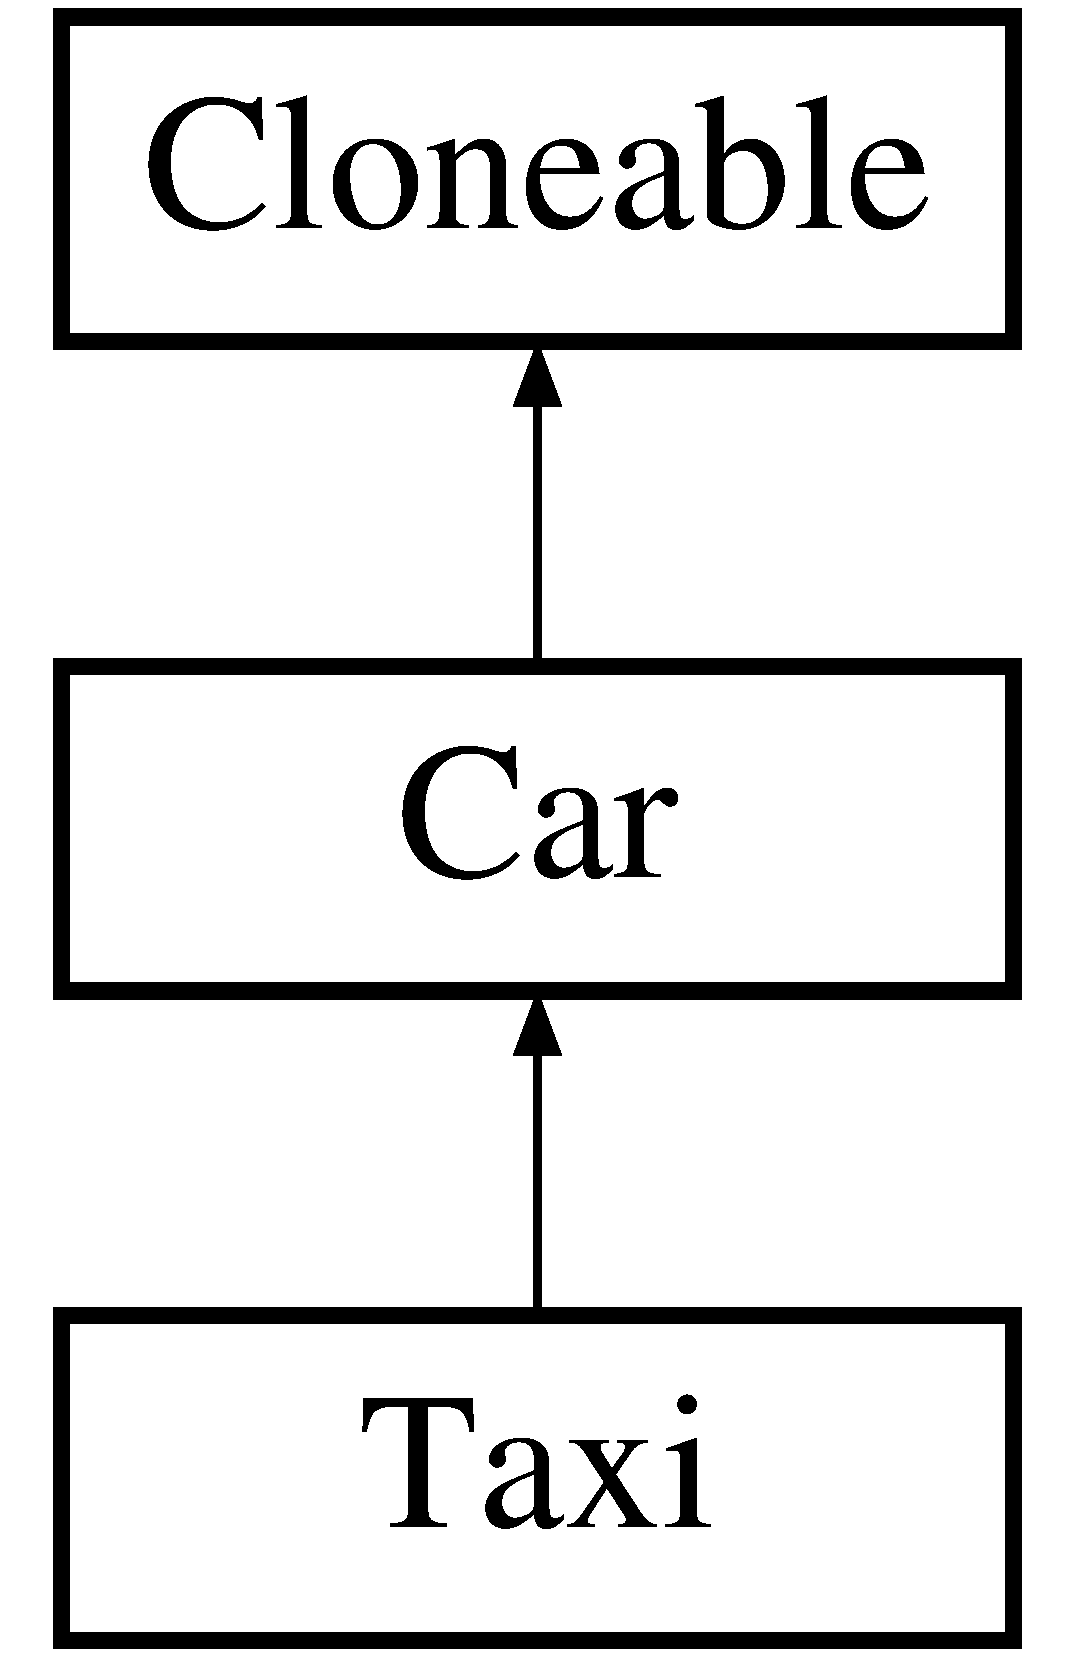
\includegraphics[height=3.000000cm]{class_car}
\end{center}
\end{figure}
\subsection*{Public Member Functions}
\begin{DoxyCompactItemize}
\item 
\hypertarget{class_car_abc94983f5c6da76940df4087acaa90c8}{void \hyperlink{class_car_abc94983f5c6da76940df4087acaa90c8}{step} ()}\label{class_car_abc94983f5c6da76940df4087acaa90c8}

\begin{DoxyCompactList}\small\item\em Steps lifetime of car, i.\+e amount of time the car has been in the simulation. \end{DoxyCompactList}\item 
\hypertarget{class_car_a3c0e698c2a1173191ee6fdb24f21e201}{void \hyperlink{class_car_a3c0e698c2a1173191ee6fdb24f21e201}{step\+Waiting\+Time} ()}\label{class_car_a3c0e698c2a1173191ee6fdb24f21e201}

\begin{DoxyCompactList}\small\item\em Steps the waiting time, i.\+e the amount of time the car has been waiting for traffic lights or due to queues. \end{DoxyCompactList}\item 
\hyperlink{class_car_a7dbb44fc230f48c8482f48187da025ca}{Car} (int \hyperlink{class_car_a6c77e5ff6ce04822eca2d7b246d3b516}{lifetime}, \hyperlink{class_car_position}{Car\+Position} \hyperlink{class_car_a8ec85c8488be9a19f14077fb861b7753}{destination}, int \hyperlink{class_car_afde6b5c1b796970c1c57c3039058b731}{car\+Nr})
\begin{DoxyCompactList}\small\item\em Instantiates a new car. \end{DoxyCompactList}\item 
\hyperlink{class_car_af2ee886c2de97f28065affbfe4fe88ef}{Car} (int \hyperlink{class_car_a6c77e5ff6ce04822eca2d7b246d3b516}{lifetime}, int \hyperlink{class_car_afde6b5c1b796970c1c57c3039058b731}{car\+Nr})
\begin{DoxyCompactList}\small\item\em Instantiates a new car. \end{DoxyCompactList}\item 
\hypertarget{class_car_ad3b361d4b20d3d13034f964eb023e213}{\hyperlink{class_car}{Car} {\bfseries clone} ()  throws Clone\+Not\+Supported\+Exception}\label{class_car_ad3b361d4b20d3d13034f964eb023e213}

\item 
\hypertarget{class_car_ab6c6c319f2d635748b34c0e24596feca}{void \hyperlink{class_car_ab6c6c319f2d635748b34c0e24596feca}{set\+Finished} ()}\label{class_car_ab6c6c319f2d635748b34c0e24596feca}

\begin{DoxyCompactList}\small\item\em Sets a car to finished. \end{DoxyCompactList}\item 
boolean \hyperlink{class_car_ac66efad04dca42f1dac6f9d4421f283f}{is\+Finished} ()
\begin{DoxyCompactList}\small\item\em Checks if a car has been set to finished, i.\+e is finished with the simulation. \end{DoxyCompactList}\item 
void \hyperlink{class_car_a966437af777f1187194ffcca3a4707fd}{random\+Destination} (\hyperlink{class_car_position}{Car\+Position} s1, \hyperlink{class_car_position}{Car\+Position} s2)
\begin{DoxyCompactList}\small\item\em Generates a random destination for the car to reach. \end{DoxyCompactList}\item 
void \hyperlink{class_car_a82739f8a2cd5feb3d41fbb386ed4539a}{set\+Position} (\hyperlink{class_car_position}{Car\+Position} \hyperlink{class_car_aa2011891bfead81fe201257172843a95}{current\+Position})
\begin{DoxyCompactList}\small\item\em Sets the position of the car. \end{DoxyCompactList}\item 
\hyperlink{class_car_position}{Car\+Position} \hyperlink{class_car_ab3350ba59a2a0f54866dc525a5f3d453}{get\+Position} ()
\begin{DoxyCompactList}\small\item\em Gets the position of the car. \end{DoxyCompactList}\item 
int \hyperlink{class_car_aa576cf15525523b1fff309555bb091de}{get\+Car\+Nr} ()
\begin{DoxyCompactList}\small\item\em Gets the car number. \end{DoxyCompactList}\item 
void \hyperlink{class_car_a749a0f1dd5d45ade9997f9d349376df2}{set\+Destination} (\hyperlink{class_car_position}{Car\+Position} \hyperlink{class_car_a8ec85c8488be9a19f14077fb861b7753}{destination})
\begin{DoxyCompactList}\small\item\em Sets the destination of the car to be reached. \end{DoxyCompactList}\item 
\hyperlink{class_car_position}{Car\+Position} \hyperlink{class_car_a24a7acc04b4ff363cd60c2dc8c0e5d26}{get\+Destination} ()
\begin{DoxyCompactList}\small\item\em Gets the car destination. \end{DoxyCompactList}\item 
void \hyperlink{class_car_ad654f48f8504b657ecaa866d90322513}{set\+Int\+Position} (int i)
\begin{DoxyCompactList}\small\item\em Sets the integer position of the car. \end{DoxyCompactList}\item 
int \hyperlink{class_car_ad6318c766e3d7235a3c75eaf71f3fd16}{get\+Int\+Position} ()
\begin{DoxyCompactList}\small\item\em Gets the position of the car in integer format to be used for printing purposes. \end{DoxyCompactList}\item 
int \hyperlink{class_car_a2b19b4d99199a18d4c331089164b2dc9}{get\+Waiting\+Time} ()
\begin{DoxyCompactList}\small\item\em Gets the waiting time of the car. \end{DoxyCompactList}\item 
String \hyperlink{class_car_a164ed12b81b460e2ef43f038f1aa6319}{to\+String\+Car} ()
\begin{DoxyCompactList}\small\item\em Prints data about the car. \end{DoxyCompactList}\end{DoxyCompactItemize}
\subsection*{Protected Attributes}
\begin{DoxyCompactItemize}
\item 
int \hyperlink{class_car_afde6b5c1b796970c1c57c3039058b731}{car\+Nr}
\begin{DoxyCompactList}\small\item\em The car number. \end{DoxyCompactList}\item 
int \hyperlink{class_car_a6c77e5ff6ce04822eca2d7b246d3b516}{lifetime}
\begin{DoxyCompactList}\small\item\em The lifetime of the car. \end{DoxyCompactList}\item 
\hyperlink{class_car_position}{Car\+Position} \hyperlink{class_car_a8ec85c8488be9a19f14077fb861b7753}{destination}
\begin{DoxyCompactList}\small\item\em The destination of the car (Forward or turn). \end{DoxyCompactList}\item 
int \hyperlink{class_car_a37c19f61aed67e2b9ec340f5ef4f99bd}{int\+Position}
\begin{DoxyCompactList}\small\item\em The integer position of the car, used for printing purposes. \end{DoxyCompactList}\item 
\hyperlink{class_car_position}{Car\+Position} \hyperlink{class_car_aa2011891bfead81fe201257172843a95}{current\+Position}
\begin{DoxyCompactList}\small\item\em The current position. \end{DoxyCompactList}\item 
int \hyperlink{class_car_a523ff2c3f03e44be3ca40596f8e0ca43}{waiting\+Time} = 0
\begin{DoxyCompactList}\small\item\em The amount of time the car has been waiting at traffic lights or due to queues. \end{DoxyCompactList}\item 
boolean \hyperlink{class_car_aefe0e86fc27b1175e338447493c169a4}{route\+Finished} = false
\begin{DoxyCompactList}\small\item\em Boolean to be set to true when the car has reached its destination. \end{DoxyCompactList}\item 
String \hyperlink{class_car_a94ad7e01cd9c699c28bd77b773b883fe}{string\+Destination}
\begin{DoxyCompactList}\small\item\em String destination, used for printing purposes. \end{DoxyCompactList}\end{DoxyCompactItemize}


\subsection{Detailed Description}
The Class \hyperlink{class_car}{Car}. 

\subsection{Constructor \& Destructor Documentation}
\hypertarget{class_car_a7dbb44fc230f48c8482f48187da025ca}{\index{Car@{Car}!Car@{Car}}
\index{Car@{Car}!Car@{Car}}
\subsubsection[{Car}]{\setlength{\rightskip}{0pt plus 5cm}Car.\+Car (
\begin{DoxyParamCaption}
\item[{int}]{lifetime, }
\item[{{\bf Car\+Position}}]{destination, }
\item[{int}]{car\+Nr}
\end{DoxyParamCaption}
)}}\label{class_car_a7dbb44fc230f48c8482f48187da025ca}


Instantiates a new car. 


\begin{DoxyParams}{Parameters}
{\em lifetime} & the lifetime \\
\hline
{\em destination} & the destination \\
\hline
{\em car\+Nr} & the car nr \\
\hline
\end{DoxyParams}
\hypertarget{class_car_af2ee886c2de97f28065affbfe4fe88ef}{\index{Car@{Car}!Car@{Car}}
\index{Car@{Car}!Car@{Car}}
\subsubsection[{Car}]{\setlength{\rightskip}{0pt plus 5cm}Car.\+Car (
\begin{DoxyParamCaption}
\item[{int}]{lifetime, }
\item[{int}]{car\+Nr}
\end{DoxyParamCaption}
)}}\label{class_car_af2ee886c2de97f28065affbfe4fe88ef}


Instantiates a new car. 


\begin{DoxyParams}{Parameters}
{\em lifetime} & the lifetime \\
\hline
{\em car\+Nr} & the car number \\
\hline
\end{DoxyParams}


\subsection{Member Function Documentation}
\hypertarget{class_car_aa576cf15525523b1fff309555bb091de}{\index{Car@{Car}!get\+Car\+Nr@{get\+Car\+Nr}}
\index{get\+Car\+Nr@{get\+Car\+Nr}!Car@{Car}}
\subsubsection[{get\+Car\+Nr}]{\setlength{\rightskip}{0pt plus 5cm}int Car.\+get\+Car\+Nr (
\begin{DoxyParamCaption}
{}
\end{DoxyParamCaption}
)}}\label{class_car_aa576cf15525523b1fff309555bb091de}


Gets the car number. 

\begin{DoxyReturn}{Returns}
the car number 
\end{DoxyReturn}
\hypertarget{class_car_a24a7acc04b4ff363cd60c2dc8c0e5d26}{\index{Car@{Car}!get\+Destination@{get\+Destination}}
\index{get\+Destination@{get\+Destination}!Car@{Car}}
\subsubsection[{get\+Destination}]{\setlength{\rightskip}{0pt plus 5cm}{\bf Car\+Position} Car.\+get\+Destination (
\begin{DoxyParamCaption}
{}
\end{DoxyParamCaption}
)}}\label{class_car_a24a7acc04b4ff363cd60c2dc8c0e5d26}


Gets the car destination. 

\begin{DoxyReturn}{Returns}
the destination 
\end{DoxyReturn}
\hypertarget{class_car_ad6318c766e3d7235a3c75eaf71f3fd16}{\index{Car@{Car}!get\+Int\+Position@{get\+Int\+Position}}
\index{get\+Int\+Position@{get\+Int\+Position}!Car@{Car}}
\subsubsection[{get\+Int\+Position}]{\setlength{\rightskip}{0pt plus 5cm}int Car.\+get\+Int\+Position (
\begin{DoxyParamCaption}
{}
\end{DoxyParamCaption}
)}}\label{class_car_ad6318c766e3d7235a3c75eaf71f3fd16}


Gets the position of the car in integer format to be used for printing purposes. 

\begin{DoxyReturn}{Returns}
the int position 
\end{DoxyReturn}
\hypertarget{class_car_ab3350ba59a2a0f54866dc525a5f3d453}{\index{Car@{Car}!get\+Position@{get\+Position}}
\index{get\+Position@{get\+Position}!Car@{Car}}
\subsubsection[{get\+Position}]{\setlength{\rightskip}{0pt plus 5cm}{\bf Car\+Position} Car.\+get\+Position (
\begin{DoxyParamCaption}
{}
\end{DoxyParamCaption}
)}}\label{class_car_ab3350ba59a2a0f54866dc525a5f3d453}


Gets the position of the car. 

\begin{DoxyReturn}{Returns}
The position 
\end{DoxyReturn}
\hypertarget{class_car_a2b19b4d99199a18d4c331089164b2dc9}{\index{Car@{Car}!get\+Waiting\+Time@{get\+Waiting\+Time}}
\index{get\+Waiting\+Time@{get\+Waiting\+Time}!Car@{Car}}
\subsubsection[{get\+Waiting\+Time}]{\setlength{\rightskip}{0pt plus 5cm}int Car.\+get\+Waiting\+Time (
\begin{DoxyParamCaption}
{}
\end{DoxyParamCaption}
)}}\label{class_car_a2b19b4d99199a18d4c331089164b2dc9}


Gets the waiting time of the car. 

\begin{DoxyReturn}{Returns}
the waiting time 
\end{DoxyReturn}
\hypertarget{class_car_ac66efad04dca42f1dac6f9d4421f283f}{\index{Car@{Car}!is\+Finished@{is\+Finished}}
\index{is\+Finished@{is\+Finished}!Car@{Car}}
\subsubsection[{is\+Finished}]{\setlength{\rightskip}{0pt plus 5cm}boolean Car.\+is\+Finished (
\begin{DoxyParamCaption}
{}
\end{DoxyParamCaption}
)}}\label{class_car_ac66efad04dca42f1dac6f9d4421f283f}


Checks if a car has been set to finished, i.\+e is finished with the simulation. 

\begin{DoxyReturn}{Returns}
true, if finished 
\end{DoxyReturn}
\hypertarget{class_car_a966437af777f1187194ffcca3a4707fd}{\index{Car@{Car}!random\+Destination@{random\+Destination}}
\index{random\+Destination@{random\+Destination}!Car@{Car}}
\subsubsection[{random\+Destination}]{\setlength{\rightskip}{0pt plus 5cm}void Car.\+random\+Destination (
\begin{DoxyParamCaption}
\item[{{\bf Car\+Position}}]{s1, }
\item[{{\bf Car\+Position}}]{s2}
\end{DoxyParamCaption}
)}}\label{class_car_a966437af777f1187194ffcca3a4707fd}


Generates a random destination for the car to reach. 


\begin{DoxyParams}{Parameters}
{\em s1} & forward \\
\hline
{\em s2} & turn \\
\hline
\end{DoxyParams}
\hypertarget{class_car_a749a0f1dd5d45ade9997f9d349376df2}{\index{Car@{Car}!set\+Destination@{set\+Destination}}
\index{set\+Destination@{set\+Destination}!Car@{Car}}
\subsubsection[{set\+Destination}]{\setlength{\rightskip}{0pt plus 5cm}void Car.\+set\+Destination (
\begin{DoxyParamCaption}
\item[{{\bf Car\+Position}}]{destination}
\end{DoxyParamCaption}
)}}\label{class_car_a749a0f1dd5d45ade9997f9d349376df2}


Sets the destination of the car to be reached. 


\begin{DoxyParams}{Parameters}
{\em destination} & the new destination \\
\hline
\end{DoxyParams}
\hypertarget{class_car_ad654f48f8504b657ecaa866d90322513}{\index{Car@{Car}!set\+Int\+Position@{set\+Int\+Position}}
\index{set\+Int\+Position@{set\+Int\+Position}!Car@{Car}}
\subsubsection[{set\+Int\+Position}]{\setlength{\rightskip}{0pt plus 5cm}void Car.\+set\+Int\+Position (
\begin{DoxyParamCaption}
\item[{int}]{i}
\end{DoxyParamCaption}
)}}\label{class_car_ad654f48f8504b657ecaa866d90322513}


Sets the integer position of the car. 


\begin{DoxyParams}{Parameters}
{\em i} & the new integer position \\
\hline
\end{DoxyParams}
\hypertarget{class_car_a82739f8a2cd5feb3d41fbb386ed4539a}{\index{Car@{Car}!set\+Position@{set\+Position}}
\index{set\+Position@{set\+Position}!Car@{Car}}
\subsubsection[{set\+Position}]{\setlength{\rightskip}{0pt plus 5cm}void Car.\+set\+Position (
\begin{DoxyParamCaption}
\item[{{\bf Car\+Position}}]{current\+Position}
\end{DoxyParamCaption}
)}}\label{class_car_a82739f8a2cd5feb3d41fbb386ed4539a}


Sets the position of the car. 


\begin{DoxyParams}{Parameters}
{\em current\+Position} & The position \\
\hline
\end{DoxyParams}
\hypertarget{class_car_a164ed12b81b460e2ef43f038f1aa6319}{\index{Car@{Car}!to\+String\+Car@{to\+String\+Car}}
\index{to\+String\+Car@{to\+String\+Car}!Car@{Car}}
\subsubsection[{to\+String\+Car}]{\setlength{\rightskip}{0pt plus 5cm}String Car.\+to\+String\+Car (
\begin{DoxyParamCaption}
{}
\end{DoxyParamCaption}
)}}\label{class_car_a164ed12b81b460e2ef43f038f1aa6319}


Prints data about the car. 

\begin{DoxyReturn}{Returns}
the string 
\end{DoxyReturn}


\subsection{Member Data Documentation}
\hypertarget{class_car_afde6b5c1b796970c1c57c3039058b731}{\index{Car@{Car}!car\+Nr@{car\+Nr}}
\index{car\+Nr@{car\+Nr}!Car@{Car}}
\subsubsection[{car\+Nr}]{\setlength{\rightskip}{0pt plus 5cm}int Car.\+car\+Nr\hspace{0.3cm}{\ttfamily [protected]}}}\label{class_car_afde6b5c1b796970c1c57c3039058b731}


The car number. 

\hypertarget{class_car_aa2011891bfead81fe201257172843a95}{\index{Car@{Car}!current\+Position@{current\+Position}}
\index{current\+Position@{current\+Position}!Car@{Car}}
\subsubsection[{current\+Position}]{\setlength{\rightskip}{0pt plus 5cm}{\bf Car\+Position} Car.\+current\+Position\hspace{0.3cm}{\ttfamily [protected]}}}\label{class_car_aa2011891bfead81fe201257172843a95}


The current position. 

\hypertarget{class_car_a8ec85c8488be9a19f14077fb861b7753}{\index{Car@{Car}!destination@{destination}}
\index{destination@{destination}!Car@{Car}}
\subsubsection[{destination}]{\setlength{\rightskip}{0pt plus 5cm}{\bf Car\+Position} Car.\+destination\hspace{0.3cm}{\ttfamily [protected]}}}\label{class_car_a8ec85c8488be9a19f14077fb861b7753}


The destination of the car (Forward or turn). 

\hypertarget{class_car_a37c19f61aed67e2b9ec340f5ef4f99bd}{\index{Car@{Car}!int\+Position@{int\+Position}}
\index{int\+Position@{int\+Position}!Car@{Car}}
\subsubsection[{int\+Position}]{\setlength{\rightskip}{0pt plus 5cm}int Car.\+int\+Position\hspace{0.3cm}{\ttfamily [protected]}}}\label{class_car_a37c19f61aed67e2b9ec340f5ef4f99bd}


The integer position of the car, used for printing purposes. 

\hypertarget{class_car_a6c77e5ff6ce04822eca2d7b246d3b516}{\index{Car@{Car}!lifetime@{lifetime}}
\index{lifetime@{lifetime}!Car@{Car}}
\subsubsection[{lifetime}]{\setlength{\rightskip}{0pt plus 5cm}int Car.\+lifetime\hspace{0.3cm}{\ttfamily [protected]}}}\label{class_car_a6c77e5ff6ce04822eca2d7b246d3b516}


The lifetime of the car. 

\hypertarget{class_car_aefe0e86fc27b1175e338447493c169a4}{\index{Car@{Car}!route\+Finished@{route\+Finished}}
\index{route\+Finished@{route\+Finished}!Car@{Car}}
\subsubsection[{route\+Finished}]{\setlength{\rightskip}{0pt plus 5cm}boolean Car.\+route\+Finished = false\hspace{0.3cm}{\ttfamily [protected]}}}\label{class_car_aefe0e86fc27b1175e338447493c169a4}


Boolean to be set to true when the car has reached its destination. 

\hypertarget{class_car_a94ad7e01cd9c699c28bd77b773b883fe}{\index{Car@{Car}!string\+Destination@{string\+Destination}}
\index{string\+Destination@{string\+Destination}!Car@{Car}}
\subsubsection[{string\+Destination}]{\setlength{\rightskip}{0pt plus 5cm}String Car.\+string\+Destination\hspace{0.3cm}{\ttfamily [protected]}}}\label{class_car_a94ad7e01cd9c699c28bd77b773b883fe}


String destination, used for printing purposes. 

\hypertarget{class_car_a523ff2c3f03e44be3ca40596f8e0ca43}{\index{Car@{Car}!waiting\+Time@{waiting\+Time}}
\index{waiting\+Time@{waiting\+Time}!Car@{Car}}
\subsubsection[{waiting\+Time}]{\setlength{\rightskip}{0pt plus 5cm}int Car.\+waiting\+Time = 0\hspace{0.3cm}{\ttfamily [protected]}}}\label{class_car_a523ff2c3f03e44be3ca40596f8e0ca43}


The amount of time the car has been waiting at traffic lights or due to queues. 



The documentation for this class was generated from the following file\+:\begin{DoxyCompactItemize}
\item 
Car.\+java\end{DoxyCompactItemize}

\hypertarget{class_car_position}{\section{Car\+Position Class Reference}
\label{class_car_position}\index{Car\+Position@{Car\+Position}}
}


The Class \hyperlink{class_car_position}{Car\+Position}.  


\subsection*{Public Member Functions}
\begin{DoxyCompactItemize}
\item 
\hyperlink{class_car_position_a05ba9c48ae0dc6bcc7bef617e370ae77}{Car\+Position} (final \hyperlink{class_lane}{Lane} owner)
\begin{DoxyCompactList}\small\item\em Instantiates a new car position. \end{DoxyCompactList}\item 
boolean \hyperlink{class_car_position_ac7b16dd1c871461b96e3a90ab96c9323}{is\+End} (\hyperlink{class_car_position}{Car\+Position} target)
\begin{DoxyCompactList}\small\item\em Checks if the \hyperlink{class_car_position}{Car\+Position} is at the end of a \hyperlink{class_lane}{Lane}. \end{DoxyCompactList}\item 
boolean \hyperlink{class_car_position_a060a8a0043d119878c1a35af6b42291a}{move\+Forward} ()
\begin{DoxyCompactList}\small\item\em Moves the current car forward if the destination is to move forward and it's the end of the main lane. \end{DoxyCompactList}\item 
boolean \hyperlink{class_car_position_a3a07aa3135efaf79cc05273de3d0eed9}{turn} ()
\begin{DoxyCompactList}\small\item\em Moves the current car to the turning lane if the destination is to turn and it's the end of the main lane. \end{DoxyCompactList}\item 
\hyperlink{class_car}{Car} \hyperlink{class_car_position_a7f67bb341d15a5d2dfdfb4958e09e96a}{get} ()
\begin{DoxyCompactList}\small\item\em Gets the current car at the \hyperlink{class_car_position}{Car\+Position}. \end{DoxyCompactList}\item 
void \hyperlink{class_car_position_abfa74c31e5ca43d0c2c06f637ee8533f}{set\+Turn} (\hyperlink{class_car_position}{Car\+Position} turn)
\begin{DoxyCompactList}\small\item\em Updates \hyperlink{class_car_position}{Car\+Position} to turn. \end{DoxyCompactList}\item 
\hyperlink{class_car_position}{Car\+Position} \hyperlink{class_car_position_a01b5b7e2cb4c51114e3f42e7fa150c74}{get\+Turn} ()
\begin{DoxyCompactList}\small\item\em Gets the \hyperlink{class_car_position}{Car\+Position} turn. \end{DoxyCompactList}\item 
\hyperlink{class_car_position}{Car\+Position} \hyperlink{class_car_position_a4238bc30010dbc3c079fe319809f9829}{get\+Forward} ()
\begin{DoxyCompactList}\small\item\em Gets the \hyperlink{class_car_position}{Car\+Position} forward. \end{DoxyCompactList}\item 
void \hyperlink{class_car_position_aed958712c7c0614d615e7e6693fea66d}{update\+Forward} (\hyperlink{class_car_position}{Car\+Position} new\+Forward)
\begin{DoxyCompactList}\small\item\em Updates \hyperlink{class_car_position}{Car\+Position} to forward. \end{DoxyCompactList}\item 
boolean \hyperlink{class_car_position_a74eb829a0810b734335cffa0eb7942f6}{is\+There\+A\+Car} ()
\begin{DoxyCompactList}\small\item\em Checks if there's a car at the current \hyperlink{class_car_position}{Car\+Position}. \end{DoxyCompactList}\item 
void \hyperlink{class_car_position_acd286a6c991daf457a5c4bf8e166d5bc}{set} (\hyperlink{class_car}{Car} c)
\begin{DoxyCompactList}\small\item\em Sets the current car at the \hyperlink{class_car_position}{Car\+Position} to c. \end{DoxyCompactList}\item 
\hypertarget{class_car_position_af6c2c343220e88c043b1ee80b29854a3}{void \hyperlink{class_car_position_af6c2c343220e88c043b1ee80b29854a3}{set\+Null} ()}\label{class_car_position_af6c2c343220e88c043b1ee80b29854a3}

\begin{DoxyCompactList}\small\item\em Sets the current car at the \hyperlink{class_car_position}{Car\+Position} to null. \end{DoxyCompactList}\item 
int \hyperlink{class_car_position_a7e3c9cde5c517a9698f01572c4e26281}{get\+Position} ()
\begin{DoxyCompactList}\small\item\em Gets the Car\+Positions' position. \end{DoxyCompactList}\item 
void \hyperlink{class_car_position_a23d9916eb4f84d47c30980de5d0cd0be}{set\+Position} (int pos)
\begin{DoxyCompactList}\small\item\em Sets the Car\+Positions' position. \end{DoxyCompactList}\end{DoxyCompactItemize}


\subsection{Detailed Description}
The Class \hyperlink{class_car_position}{Car\+Position}. 

\subsection{Constructor \& Destructor Documentation}
\hypertarget{class_car_position_a05ba9c48ae0dc6bcc7bef617e370ae77}{\index{Car\+Position@{Car\+Position}!Car\+Position@{Car\+Position}}
\index{Car\+Position@{Car\+Position}!Car\+Position@{Car\+Position}}
\subsubsection[{Car\+Position}]{\setlength{\rightskip}{0pt plus 5cm}Car\+Position.\+Car\+Position (
\begin{DoxyParamCaption}
\item[{final {\bf Lane}}]{owner}
\end{DoxyParamCaption}
)}}\label{class_car_position_a05ba9c48ae0dc6bcc7bef617e370ae77}


Instantiates a new car position. 


\begin{DoxyParams}{Parameters}
{\em owner} & the lane which the \hyperlink{class_car_position}{Car\+Position} belongs to. \\
\hline
\end{DoxyParams}


\subsection{Member Function Documentation}
\hypertarget{class_car_position_a7f67bb341d15a5d2dfdfb4958e09e96a}{\index{Car\+Position@{Car\+Position}!get@{get}}
\index{get@{get}!Car\+Position@{Car\+Position}}
\subsubsection[{get}]{\setlength{\rightskip}{0pt plus 5cm}{\bf Car} Car\+Position.\+get (
\begin{DoxyParamCaption}
{}
\end{DoxyParamCaption}
)}}\label{class_car_position_a7f67bb341d15a5d2dfdfb4958e09e96a}


Gets the current car at the \hyperlink{class_car_position}{Car\+Position}. 

\begin{DoxyReturn}{Returns}
the current car 
\end{DoxyReturn}
\hypertarget{class_car_position_a4238bc30010dbc3c079fe319809f9829}{\index{Car\+Position@{Car\+Position}!get\+Forward@{get\+Forward}}
\index{get\+Forward@{get\+Forward}!Car\+Position@{Car\+Position}}
\subsubsection[{get\+Forward}]{\setlength{\rightskip}{0pt plus 5cm}{\bf Car\+Position} Car\+Position.\+get\+Forward (
\begin{DoxyParamCaption}
{}
\end{DoxyParamCaption}
)}}\label{class_car_position_a4238bc30010dbc3c079fe319809f9829}


Gets the \hyperlink{class_car_position}{Car\+Position} forward. 

\begin{DoxyReturn}{Returns}
forward 
\end{DoxyReturn}
\hypertarget{class_car_position_a7e3c9cde5c517a9698f01572c4e26281}{\index{Car\+Position@{Car\+Position}!get\+Position@{get\+Position}}
\index{get\+Position@{get\+Position}!Car\+Position@{Car\+Position}}
\subsubsection[{get\+Position}]{\setlength{\rightskip}{0pt plus 5cm}int Car\+Position.\+get\+Position (
\begin{DoxyParamCaption}
{}
\end{DoxyParamCaption}
)}}\label{class_car_position_a7e3c9cde5c517a9698f01572c4e26281}


Gets the Car\+Positions' position. 

\begin{DoxyReturn}{Returns}
the position 
\end{DoxyReturn}
\hypertarget{class_car_position_a01b5b7e2cb4c51114e3f42e7fa150c74}{\index{Car\+Position@{Car\+Position}!get\+Turn@{get\+Turn}}
\index{get\+Turn@{get\+Turn}!Car\+Position@{Car\+Position}}
\subsubsection[{get\+Turn}]{\setlength{\rightskip}{0pt plus 5cm}{\bf Car\+Position} Car\+Position.\+get\+Turn (
\begin{DoxyParamCaption}
{}
\end{DoxyParamCaption}
)}}\label{class_car_position_a01b5b7e2cb4c51114e3f42e7fa150c74}


Gets the \hyperlink{class_car_position}{Car\+Position} turn. 

\begin{DoxyReturn}{Returns}
turn 
\end{DoxyReturn}
\hypertarget{class_car_position_ac7b16dd1c871461b96e3a90ab96c9323}{\index{Car\+Position@{Car\+Position}!is\+End@{is\+End}}
\index{is\+End@{is\+End}!Car\+Position@{Car\+Position}}
\subsubsection[{is\+End}]{\setlength{\rightskip}{0pt plus 5cm}boolean Car\+Position.\+is\+End (
\begin{DoxyParamCaption}
\item[{{\bf Car\+Position}}]{target}
\end{DoxyParamCaption}
)}}\label{class_car_position_ac7b16dd1c871461b96e3a90ab96c9323}


Checks if the \hyperlink{class_car_position}{Car\+Position} is at the end of a \hyperlink{class_lane}{Lane}. 


\begin{DoxyParams}{Parameters}
{\em target} & the target \\
\hline
\end{DoxyParams}
\begin{DoxyReturn}{Returns}
true, if is end 
\end{DoxyReturn}
\hypertarget{class_car_position_a74eb829a0810b734335cffa0eb7942f6}{\index{Car\+Position@{Car\+Position}!is\+There\+A\+Car@{is\+There\+A\+Car}}
\index{is\+There\+A\+Car@{is\+There\+A\+Car}!Car\+Position@{Car\+Position}}
\subsubsection[{is\+There\+A\+Car}]{\setlength{\rightskip}{0pt plus 5cm}boolean Car\+Position.\+is\+There\+A\+Car (
\begin{DoxyParamCaption}
{}
\end{DoxyParamCaption}
)}}\label{class_car_position_a74eb829a0810b734335cffa0eb7942f6}


Checks if there's a car at the current \hyperlink{class_car_position}{Car\+Position}. 

\begin{DoxyReturn}{Returns}
true, if there's a car 
\end{DoxyReturn}
\hypertarget{class_car_position_a060a8a0043d119878c1a35af6b42291a}{\index{Car\+Position@{Car\+Position}!move\+Forward@{move\+Forward}}
\index{move\+Forward@{move\+Forward}!Car\+Position@{Car\+Position}}
\subsubsection[{move\+Forward}]{\setlength{\rightskip}{0pt plus 5cm}boolean Car\+Position.\+move\+Forward (
\begin{DoxyParamCaption}
{}
\end{DoxyParamCaption}
)}}\label{class_car_position_a060a8a0043d119878c1a35af6b42291a}


Moves the current car forward if the destination is to move forward and it's the end of the main lane. 

\begin{DoxyReturn}{Returns}
true, if the current car has the destination forward and is at the end of the main lane 
\end{DoxyReturn}
\hypertarget{class_car_position_acd286a6c991daf457a5c4bf8e166d5bc}{\index{Car\+Position@{Car\+Position}!set@{set}}
\index{set@{set}!Car\+Position@{Car\+Position}}
\subsubsection[{set}]{\setlength{\rightskip}{0pt plus 5cm}void Car\+Position.\+set (
\begin{DoxyParamCaption}
\item[{{\bf Car}}]{c}
\end{DoxyParamCaption}
)}}\label{class_car_position_acd286a6c991daf457a5c4bf8e166d5bc}


Sets the current car at the \hyperlink{class_car_position}{Car\+Position} to c. 


\begin{DoxyParams}{Parameters}
{\em c} & the car \\
\hline
\end{DoxyParams}
\hypertarget{class_car_position_a23d9916eb4f84d47c30980de5d0cd0be}{\index{Car\+Position@{Car\+Position}!set\+Position@{set\+Position}}
\index{set\+Position@{set\+Position}!Car\+Position@{Car\+Position}}
\subsubsection[{set\+Position}]{\setlength{\rightskip}{0pt plus 5cm}void Car\+Position.\+set\+Position (
\begin{DoxyParamCaption}
\item[{int}]{pos}
\end{DoxyParamCaption}
)}}\label{class_car_position_a23d9916eb4f84d47c30980de5d0cd0be}


Sets the Car\+Positions' position. 


\begin{DoxyParams}{Parameters}
{\em pos} & the new position \\
\hline
\end{DoxyParams}
\hypertarget{class_car_position_abfa74c31e5ca43d0c2c06f637ee8533f}{\index{Car\+Position@{Car\+Position}!set\+Turn@{set\+Turn}}
\index{set\+Turn@{set\+Turn}!Car\+Position@{Car\+Position}}
\subsubsection[{set\+Turn}]{\setlength{\rightskip}{0pt plus 5cm}void Car\+Position.\+set\+Turn (
\begin{DoxyParamCaption}
\item[{{\bf Car\+Position}}]{turn}
\end{DoxyParamCaption}
)}}\label{class_car_position_abfa74c31e5ca43d0c2c06f637ee8533f}


Updates \hyperlink{class_car_position}{Car\+Position} to turn. 


\begin{DoxyParams}{Parameters}
{\em turn} & the turn destination \\
\hline
\end{DoxyParams}
\hypertarget{class_car_position_a3a07aa3135efaf79cc05273de3d0eed9}{\index{Car\+Position@{Car\+Position}!turn@{turn}}
\index{turn@{turn}!Car\+Position@{Car\+Position}}
\subsubsection[{turn}]{\setlength{\rightskip}{0pt plus 5cm}boolean Car\+Position.\+turn (
\begin{DoxyParamCaption}
{}
\end{DoxyParamCaption}
)}}\label{class_car_position_a3a07aa3135efaf79cc05273de3d0eed9}


Moves the current car to the turning lane if the destination is to turn and it's the end of the main lane. 

\begin{DoxyReturn}{Returns}
true, if the current car has the destination turn and is at the end of the main lane 
\end{DoxyReturn}
\hypertarget{class_car_position_aed958712c7c0614d615e7e6693fea66d}{\index{Car\+Position@{Car\+Position}!update\+Forward@{update\+Forward}}
\index{update\+Forward@{update\+Forward}!Car\+Position@{Car\+Position}}
\subsubsection[{update\+Forward}]{\setlength{\rightskip}{0pt plus 5cm}void Car\+Position.\+update\+Forward (
\begin{DoxyParamCaption}
\item[{{\bf Car\+Position}}]{new\+Forward}
\end{DoxyParamCaption}
)}}\label{class_car_position_aed958712c7c0614d615e7e6693fea66d}


Updates \hyperlink{class_car_position}{Car\+Position} to forward. 


\begin{DoxyParams}{Parameters}
{\em new\+Forward} & the new forward destination \\
\hline
\end{DoxyParams}


The documentation for this class was generated from the following file\+:\begin{DoxyCompactItemize}
\item 
Car\+Position.\+java\end{DoxyCompactItemize}

\hypertarget{class_lane}{\section{Lane Class Reference}
\label{class_lane}\index{Lane@{Lane}}
}


The Class \hyperlink{class_lane}{Lane}.  


\subsection*{Public Member Functions}
\begin{DoxyCompactItemize}
\item 
\hyperlink{class_lane_a636f1d6ef695cd3ac642096c051b3d6d}{Lane} (int n)
\begin{DoxyCompactList}\small\item\em Instantiates a new lane. \end{DoxyCompactList}\item 
boolean \hyperlink{class_lane_a7a6879f035bd1fa89328914f11028ff1}{is\+Empty} ()
\begin{DoxyCompactList}\small\item\em Checks if the lane is empty. \end{DoxyCompactList}\item 
boolean \hyperlink{class_lane_a461bba912631945e1b9abceb677729a5}{match\+End} (\hyperlink{class_car_position}{Car\+Position} target)
\begin{DoxyCompactList}\small\item\em Checks whether the \hyperlink{class_car_position}{Car\+Position} target is at the end of the lane. \end{DoxyCompactList}\item 
int \hyperlink{class_lane_afc04264fa269d5be97b570890907915a}{get\+Length} ()
\begin{DoxyCompactList}\small\item\em Gets the length of the lane. \end{DoxyCompactList}\item 
\hypertarget{class_lane_a97a49d217a4db63448439a4cb013e5ca}{void {\bfseries set\+Parallel} (\hyperlink{class_lane}{Lane} side\+Lane)}\label{class_lane_a97a49d217a4db63448439a4cb013e5ca}

\item 
void \hyperlink{class_lane_a85e5eb030e32bc0825be9f3e942e5ccc}{step} ()
\begin{DoxyCompactList}\small\item\em Steps all cars in the lane one step forward if possible (except the one at position 0). \end{DoxyCompactList}\item 
\hyperlink{class_car}{Car} \hyperlink{class_lane_aac5f6634752c76e0e46358fe8dd896ba}{get\+First} ()
\begin{DoxyCompactList}\small\item\em Returns and removes the first car in the lane. \end{DoxyCompactList}\item 
\hyperlink{class_car}{Car} \hyperlink{class_lane_a9ab36dbd97899be31b4f5c28d7969e85}{first\+Car} ()
\begin{DoxyCompactList}\small\item\em Returns the first car in the lane without removing it. \end{DoxyCompactList}\item 
boolean \hyperlink{class_lane_a30c3819ef177ddab0ba45e7145babd38}{last\+Free} ()
\begin{DoxyCompactList}\small\item\em Checks whether or not the last \hyperlink{class_car_position}{Car\+Position} in the lane is free, i.\+e there's no car there. \end{DoxyCompactList}\item 
void \hyperlink{class_lane_aea316343730ee43e3dc3ba660cd46469}{put\+Last} (\hyperlink{class_car}{Car} c)  throws Overflow\+Exception 
\begin{DoxyCompactList}\small\item\em Puts the car c at the last \hyperlink{class_car_position}{Car\+Position} in the lane if it's free, otherwise throws an exception. \end{DoxyCompactList}\item 
\hypertarget{class_lane_a62510f601eff0ac72dc5f95c876a8563}{void \hyperlink{class_lane_a62510f601eff0ac72dc5f95c876a8563}{to\+String\+Lane} ()}\label{class_lane_a62510f601eff0ac72dc5f95c876a8563}

\begin{DoxyCompactList}\small\item\em Prints data about the lane. \end{DoxyCompactList}\end{DoxyCompactItemize}
\subsection*{Protected Attributes}
\begin{DoxyCompactItemize}
\item 
\hyperlink{class_car_position}{Car\+Position}\mbox{[}$\,$\mbox{]} \hyperlink{class_lane_a0e18fcb829e23827ecc2610e6e8caf0b}{the\+Lane}
\begin{DoxyCompactList}\small\item\em The lane. \end{DoxyCompactList}\item 
\hyperlink{class_car}{Car} \hyperlink{class_lane_abcd2ea6fa6aaa99b2b84e89a422c0377}{temporary\+Parking\+Spot}
\begin{DoxyCompactList}\small\item\em Temporary parking spot for cars who have reached there destination, used for statistics. \end{DoxyCompactList}\end{DoxyCompactItemize}


\subsection{Detailed Description}
The Class \hyperlink{class_lane}{Lane}. 

\subsection{Constructor \& Destructor Documentation}
\hypertarget{class_lane_a636f1d6ef695cd3ac642096c051b3d6d}{\index{Lane@{Lane}!Lane@{Lane}}
\index{Lane@{Lane}!Lane@{Lane}}
\subsubsection[{Lane}]{\setlength{\rightskip}{0pt plus 5cm}Lane.\+Lane (
\begin{DoxyParamCaption}
\item[{int}]{n}
\end{DoxyParamCaption}
)}}\label{class_lane_a636f1d6ef695cd3ac642096c051b3d6d}


Instantiates a new lane. 


\begin{DoxyParams}{Parameters}
{\em n} & the number of Car\+Positions fitting in the lane. \\
\hline
\end{DoxyParams}


\subsection{Member Function Documentation}
\hypertarget{class_lane_a9ab36dbd97899be31b4f5c28d7969e85}{\index{Lane@{Lane}!first\+Car@{first\+Car}}
\index{first\+Car@{first\+Car}!Lane@{Lane}}
\subsubsection[{first\+Car}]{\setlength{\rightskip}{0pt plus 5cm}{\bf Car} Lane.\+first\+Car (
\begin{DoxyParamCaption}
{}
\end{DoxyParamCaption}
)}}\label{class_lane_a9ab36dbd97899be31b4f5c28d7969e85}


Returns the first car in the lane without removing it. 

\begin{DoxyReturn}{Returns}
the first car 
\end{DoxyReturn}
\hypertarget{class_lane_aac5f6634752c76e0e46358fe8dd896ba}{\index{Lane@{Lane}!get\+First@{get\+First}}
\index{get\+First@{get\+First}!Lane@{Lane}}
\subsubsection[{get\+First}]{\setlength{\rightskip}{0pt plus 5cm}{\bf Car} Lane.\+get\+First (
\begin{DoxyParamCaption}
{}
\end{DoxyParamCaption}
)}}\label{class_lane_aac5f6634752c76e0e46358fe8dd896ba}


Returns and removes the first car in the lane. 

\begin{DoxyReturn}{Returns}
the first car. 
\end{DoxyReturn}
\hypertarget{class_lane_afc04264fa269d5be97b570890907915a}{\index{Lane@{Lane}!get\+Length@{get\+Length}}
\index{get\+Length@{get\+Length}!Lane@{Lane}}
\subsubsection[{get\+Length}]{\setlength{\rightskip}{0pt plus 5cm}int Lane.\+get\+Length (
\begin{DoxyParamCaption}
{}
\end{DoxyParamCaption}
)}}\label{class_lane_afc04264fa269d5be97b570890907915a}


Gets the length of the lane. 

\begin{DoxyReturn}{Returns}
the length 
\end{DoxyReturn}
\hypertarget{class_lane_a7a6879f035bd1fa89328914f11028ff1}{\index{Lane@{Lane}!is\+Empty@{is\+Empty}}
\index{is\+Empty@{is\+Empty}!Lane@{Lane}}
\subsubsection[{is\+Empty}]{\setlength{\rightskip}{0pt plus 5cm}boolean Lane.\+is\+Empty (
\begin{DoxyParamCaption}
{}
\end{DoxyParamCaption}
)}}\label{class_lane_a7a6879f035bd1fa89328914f11028ff1}


Checks if the lane is empty. 

\begin{DoxyReturn}{Returns}
true, if the lane is empty 
\end{DoxyReturn}
\hypertarget{class_lane_a30c3819ef177ddab0ba45e7145babd38}{\index{Lane@{Lane}!last\+Free@{last\+Free}}
\index{last\+Free@{last\+Free}!Lane@{Lane}}
\subsubsection[{last\+Free}]{\setlength{\rightskip}{0pt plus 5cm}boolean Lane.\+last\+Free (
\begin{DoxyParamCaption}
{}
\end{DoxyParamCaption}
)}}\label{class_lane_a30c3819ef177ddab0ba45e7145babd38}


Checks whether or not the last \hyperlink{class_car_position}{Car\+Position} in the lane is free, i.\+e there's no car there. 

\begin{DoxyReturn}{Returns}
true, if the last \hyperlink{class_car_position}{Car\+Position} is free. 
\end{DoxyReturn}
\hypertarget{class_lane_a461bba912631945e1b9abceb677729a5}{\index{Lane@{Lane}!match\+End@{match\+End}}
\index{match\+End@{match\+End}!Lane@{Lane}}
\subsubsection[{match\+End}]{\setlength{\rightskip}{0pt plus 5cm}boolean Lane.\+match\+End (
\begin{DoxyParamCaption}
\item[{{\bf Car\+Position}}]{target}
\end{DoxyParamCaption}
)}}\label{class_lane_a461bba912631945e1b9abceb677729a5}


Checks whether the \hyperlink{class_car_position}{Car\+Position} target is at the end of the lane. 


\begin{DoxyParams}{Parameters}
{\em target} & the target \hyperlink{class_car_position}{Car\+Position} \\
\hline
\end{DoxyParams}
\begin{DoxyReturn}{Returns}
true, if target is at the end of the lane 
\end{DoxyReturn}
\hypertarget{class_lane_aea316343730ee43e3dc3ba660cd46469}{\index{Lane@{Lane}!put\+Last@{put\+Last}}
\index{put\+Last@{put\+Last}!Lane@{Lane}}
\subsubsection[{put\+Last}]{\setlength{\rightskip}{0pt plus 5cm}void Lane.\+put\+Last (
\begin{DoxyParamCaption}
\item[{{\bf Car}}]{c}
\end{DoxyParamCaption}
) throws {\bf Overflow\+Exception}}}\label{class_lane_aea316343730ee43e3dc3ba660cd46469}


Puts the car c at the last \hyperlink{class_car_position}{Car\+Position} in the lane if it's free, otherwise throws an exception. 


\begin{DoxyParams}{Parameters}
{\em c} & the car \\
\hline
\end{DoxyParams}

\begin{DoxyExceptions}{Exceptions}
{\em \hyperlink{class_overflow_exception}{Overflow\+Exception}} & Overflow exception if the last \hyperlink{class_car_position}{Car\+Position} is occupied. \\
\hline
\end{DoxyExceptions}
\hypertarget{class_lane_a85e5eb030e32bc0825be9f3e942e5ccc}{\index{Lane@{Lane}!step@{step}}
\index{step@{step}!Lane@{Lane}}
\subsubsection[{step}]{\setlength{\rightskip}{0pt plus 5cm}void Lane.\+step (
\begin{DoxyParamCaption}
{}
\end{DoxyParamCaption}
)}}\label{class_lane_a85e5eb030e32bc0825be9f3e942e5ccc}


Steps all cars in the lane one step forward if possible (except the one at position 0). 

The car at position 0 gets added to the temporary\+Parting\+Spot to be used for statistics. 

\subsection{Member Data Documentation}
\hypertarget{class_lane_abcd2ea6fa6aaa99b2b84e89a422c0377}{\index{Lane@{Lane}!temporary\+Parking\+Spot@{temporary\+Parking\+Spot}}
\index{temporary\+Parking\+Spot@{temporary\+Parking\+Spot}!Lane@{Lane}}
\subsubsection[{temporary\+Parking\+Spot}]{\setlength{\rightskip}{0pt plus 5cm}{\bf Car} Lane.\+temporary\+Parking\+Spot\hspace{0.3cm}{\ttfamily [protected]}}}\label{class_lane_abcd2ea6fa6aaa99b2b84e89a422c0377}


Temporary parking spot for cars who have reached there destination, used for statistics. 

\hypertarget{class_lane_a0e18fcb829e23827ecc2610e6e8caf0b}{\index{Lane@{Lane}!the\+Lane@{the\+Lane}}
\index{the\+Lane@{the\+Lane}!Lane@{Lane}}
\subsubsection[{the\+Lane}]{\setlength{\rightskip}{0pt plus 5cm}{\bf Car\+Position} \mbox{[}$\,$\mbox{]} Lane.\+the\+Lane\hspace{0.3cm}{\ttfamily [protected]}}}\label{class_lane_a0e18fcb829e23827ecc2610e6e8caf0b}


The lane. 



The documentation for this class was generated from the following file\+:\begin{DoxyCompactItemize}
\item 
Lane.\+java\end{DoxyCompactItemize}

\hypertarget{class_light}{\section{Light Class Reference}
\label{class_light}\index{Light@{Light}}
}


The Class \hyperlink{class_light}{Light}.  


\subsection*{Public Member Functions}
\begin{DoxyCompactItemize}
\item 
\hyperlink{class_light_a58aae408cb21d0158eb356cc69a2aed5}{Light} (int period, int green)
\begin{DoxyCompactList}\small\item\em Instantiates a new light. \end{DoxyCompactList}\item 
\hypertarget{class_light_a713e0a8b07227041e41a56c030ce35b4}{void \hyperlink{class_light_a713e0a8b07227041e41a56c030ce35b4}{step} ()}\label{class_light_a713e0a8b07227041e41a56c030ce35b4}

\begin{DoxyCompactList}\small\item\em Increases the time by one. \end{DoxyCompactList}\item 
boolean \hyperlink{class_light_a1190182015f9e4766ce100599417cfb9}{is\+Green} ()
\begin{DoxyCompactList}\small\item\em Checks whether the traffic light is green. \end{DoxyCompactList}\item 
\hypertarget{class_light_a46458933ff24f059209f1846927637fd}{String {\bfseries to\+String} ()}\label{class_light_a46458933ff24f059209f1846927637fd}

\end{DoxyCompactItemize}


\subsection{Detailed Description}
The Class \hyperlink{class_light}{Light}. 

\subsection{Constructor \& Destructor Documentation}
\hypertarget{class_light_a58aae408cb21d0158eb356cc69a2aed5}{\index{Light@{Light}!Light@{Light}}
\index{Light@{Light}!Light@{Light}}
\subsubsection[{Light}]{\setlength{\rightskip}{0pt plus 5cm}Light.\+Light (
\begin{DoxyParamCaption}
\item[{int}]{period, }
\item[{int}]{green}
\end{DoxyParamCaption}
)}}\label{class_light_a58aae408cb21d0158eb356cc69a2aed5}


Instantiates a new light. 


\begin{DoxyParams}{Parameters}
{\em period} & the period time \\
\hline
{\em green} & the green time \\
\hline
\end{DoxyParams}


\subsection{Member Function Documentation}
\hypertarget{class_light_a1190182015f9e4766ce100599417cfb9}{\index{Light@{Light}!is\+Green@{is\+Green}}
\index{is\+Green@{is\+Green}!Light@{Light}}
\subsubsection[{is\+Green}]{\setlength{\rightskip}{0pt plus 5cm}boolean Light.\+is\+Green (
\begin{DoxyParamCaption}
{}
\end{DoxyParamCaption}
)}}\label{class_light_a1190182015f9e4766ce100599417cfb9}


Checks whether the traffic light is green. 

\begin{DoxyReturn}{Returns}
true, if the traffic light is green 
\end{DoxyReturn}


The documentation for this class was generated from the following file\+:\begin{DoxyCompactItemize}
\item 
Light.\+java\end{DoxyCompactItemize}

\hypertarget{class_overflow_exception}{\section{Overflow\+Exception Class Reference}
\label{class_overflow_exception}\index{Overflow\+Exception@{Overflow\+Exception}}
}


The Class \hyperlink{class_overflow_exception}{Overflow\+Exception}.  


Inheritance diagram for Overflow\+Exception\+:\begin{figure}[H]
\begin{center}
\leavevmode
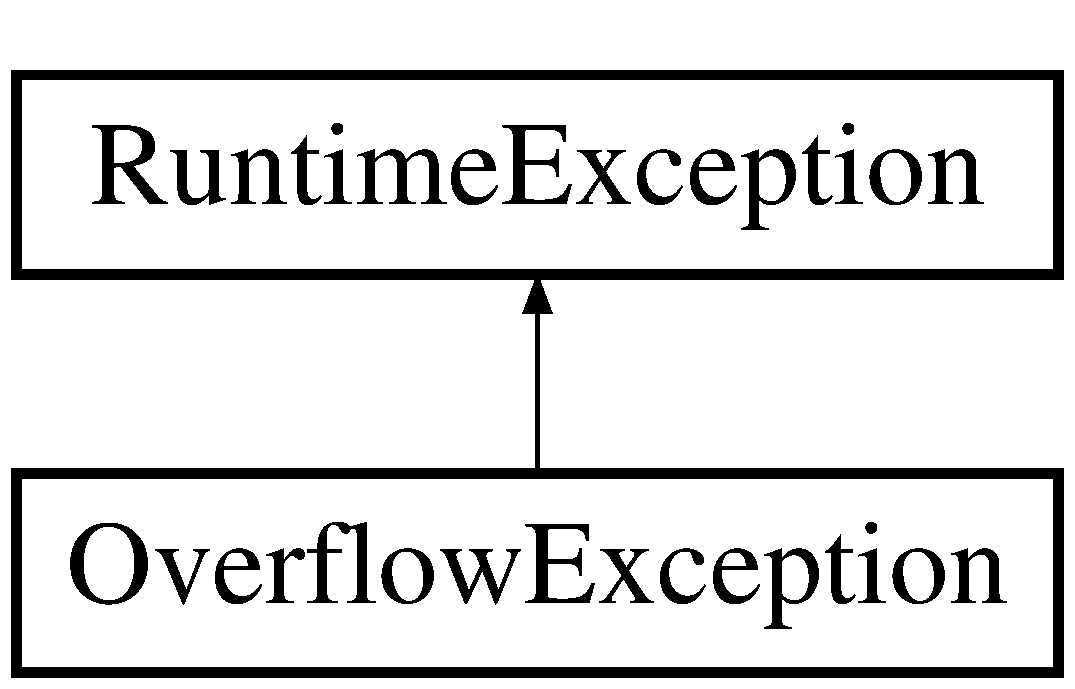
\includegraphics[height=2.000000cm]{class_overflow_exception}
\end{center}
\end{figure}
\subsection*{Public Member Functions}
\begin{DoxyCompactItemize}
\item 
\hypertarget{class_overflow_exception_aa443b9a3418c8f5b10f2b7e69d8c38ef}{\hyperlink{class_overflow_exception_aa443b9a3418c8f5b10f2b7e69d8c38ef}{Overflow\+Exception} ()}\label{class_overflow_exception_aa443b9a3418c8f5b10f2b7e69d8c38ef}

\begin{DoxyCompactList}\small\item\em Instantiates a new overflow exception. \end{DoxyCompactList}\item 
\hyperlink{class_overflow_exception_a9769bc5767762ef1c2b8c0e859d20103}{Overflow\+Exception} (String s)
\begin{DoxyCompactList}\small\item\em Instantiates a new overflow exception. \end{DoxyCompactList}\end{DoxyCompactItemize}


\subsection{Detailed Description}
The Class \hyperlink{class_overflow_exception}{Overflow\+Exception}. 

\subsection{Constructor \& Destructor Documentation}
\hypertarget{class_overflow_exception_a9769bc5767762ef1c2b8c0e859d20103}{\index{Overflow\+Exception@{Overflow\+Exception}!Overflow\+Exception@{Overflow\+Exception}}
\index{Overflow\+Exception@{Overflow\+Exception}!Overflow\+Exception@{Overflow\+Exception}}
\subsubsection[{Overflow\+Exception}]{\setlength{\rightskip}{0pt plus 5cm}Overflow\+Exception.\+Overflow\+Exception (
\begin{DoxyParamCaption}
\item[{String}]{s}
\end{DoxyParamCaption}
)}}\label{class_overflow_exception_a9769bc5767762ef1c2b8c0e859d20103}


Instantiates a new overflow exception. 


\begin{DoxyParams}{Parameters}
{\em s} & string to be printed if needed. \\
\hline
\end{DoxyParams}


The documentation for this class was generated from the following file\+:\begin{DoxyCompactItemize}
\item 
Overflow\+Exception.\+java\end{DoxyCompactItemize}

\hypertarget{class_simulation}{\section{Simulation Class Reference}
\label{class_simulation}\index{Simulation@{Simulation}}
}


The Class \hyperlink{class_simulation}{Simulation}.  


\subsection*{Static Public Member Functions}
\begin{DoxyCompactItemize}
\item 
static int\mbox{[}$\,$\mbox{]} \hyperlink{class_simulation_acb57995f9549cd479cdf87d9b707c72a}{menu} ()
\begin{DoxyCompactList}\small\item\em The main menu of the simulation. \end{DoxyCompactList}\item 
static void \hyperlink{class_simulation_af4d0a3a9e5fc09cb418b358ac9811b34}{main} (String\mbox{[}$\,$\mbox{]} args)
\begin{DoxyCompactList}\small\item\em The main method of the program which runs the simulation with the user specified input values. \end{DoxyCompactList}\end{DoxyCompactItemize}


\subsection{Detailed Description}
The Class \hyperlink{class_simulation}{Simulation}. 

\subsection{Member Function Documentation}
\hypertarget{class_simulation_af4d0a3a9e5fc09cb418b358ac9811b34}{\index{Simulation@{Simulation}!main@{main}}
\index{main@{main}!Simulation@{Simulation}}
\subsubsection[{main}]{\setlength{\rightskip}{0pt plus 5cm}static void Simulation.\+main (
\begin{DoxyParamCaption}
\item[{String\mbox{[}$\,$\mbox{]}}]{args}
\end{DoxyParamCaption}
)\hspace{0.3cm}{\ttfamily [static]}}}\label{class_simulation_af4d0a3a9e5fc09cb418b358ac9811b34}


The main method of the program which runs the simulation with the user specified input values. 

Flushes the terminal screen and initiates the simulation countdown. \hypertarget{class_simulation_acb57995f9549cd479cdf87d9b707c72a}{\index{Simulation@{Simulation}!menu@{menu}}
\index{menu@{menu}!Simulation@{Simulation}}
\subsubsection[{menu}]{\setlength{\rightskip}{0pt plus 5cm}static int \mbox{[}$\,$\mbox{]} Simulation.\+menu (
\begin{DoxyParamCaption}
{}
\end{DoxyParamCaption}
)\hspace{0.3cm}{\ttfamily [static]}}}\label{class_simulation_acb57995f9549cd479cdf87d9b707c72a}


The main menu of the simulation. 

Welcomes and asks the user for values to be executed. The input values are\+: length of main road, length of turning lane, red and green light periods, amount of cars to be simulated and the simulation speed.

\begin{DoxyReturn}{Returns}
all input values as an integer array 
\end{DoxyReturn}


The documentation for this class was generated from the following file\+:\begin{DoxyCompactItemize}
\item 
Simulation.\+java\end{DoxyCompactItemize}

\hypertarget{class_taxi}{\section{Taxi Class Reference}
\label{class_taxi}\index{Taxi@{Taxi}}
}


The Class \hyperlink{class_taxi}{Taxi}.  


Inheritance diagram for Taxi\+:\begin{figure}[H]
\begin{center}
\leavevmode
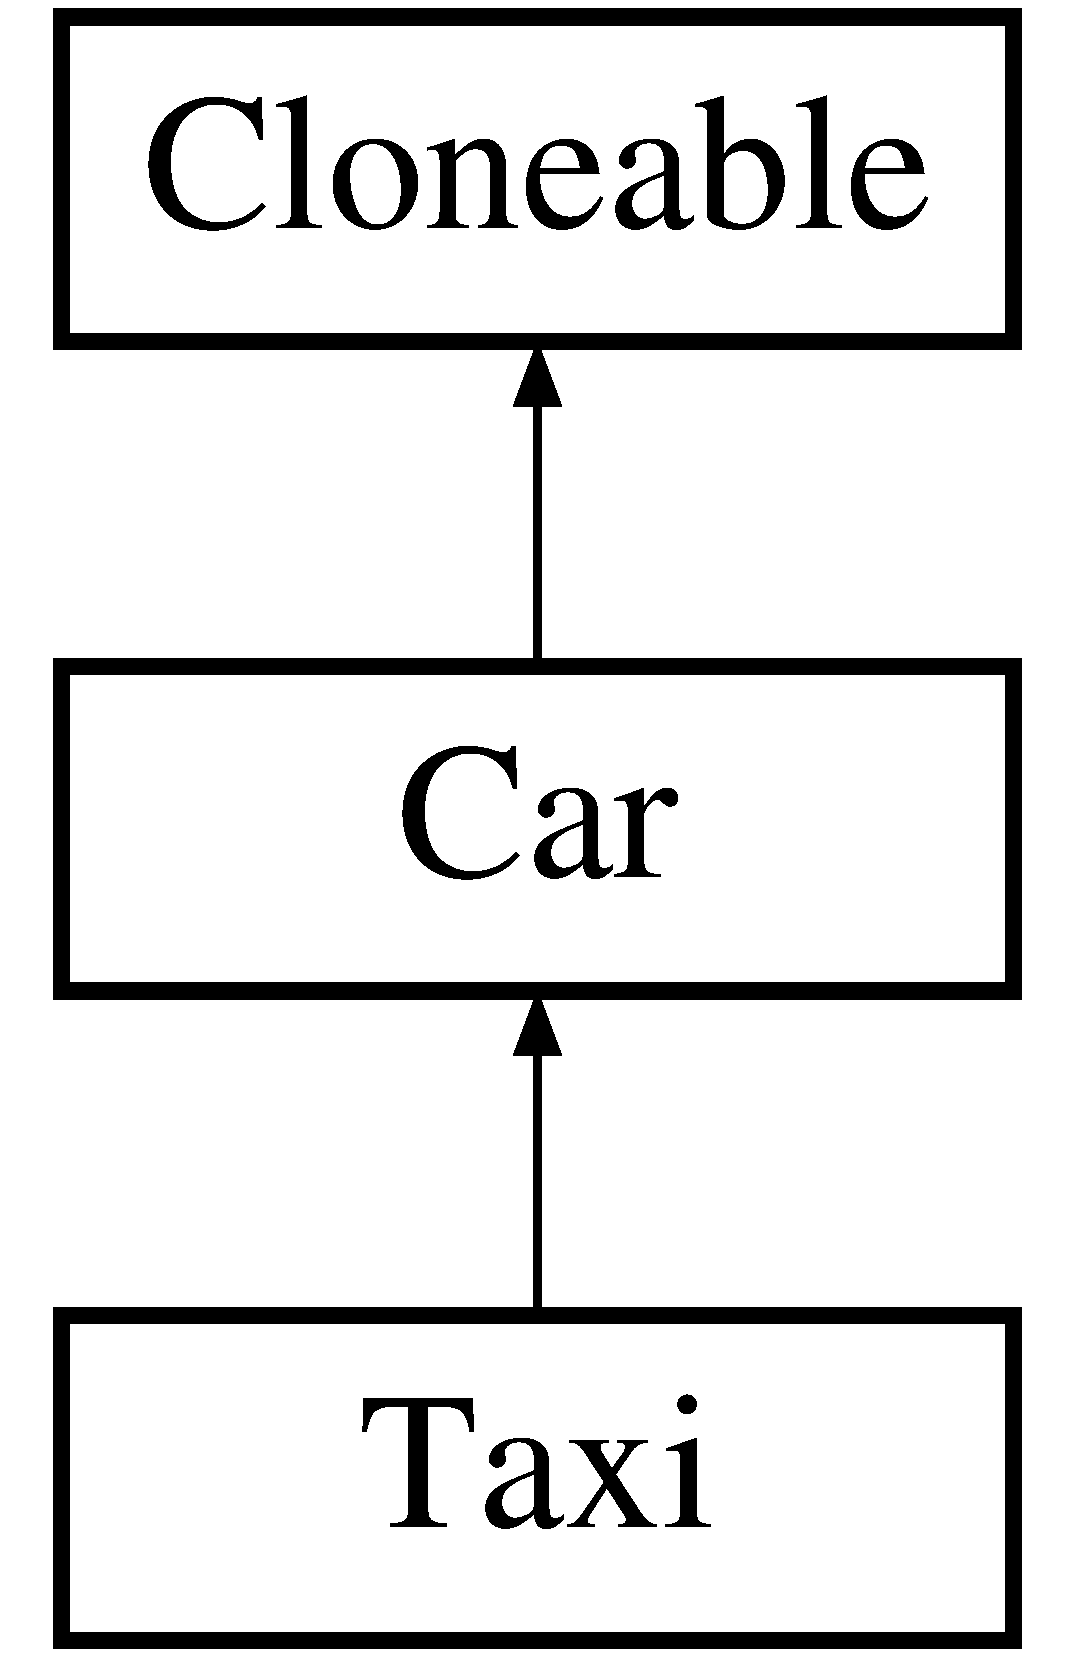
\includegraphics[height=3.000000cm]{class_taxi}
\end{center}
\end{figure}
\subsection*{Public Member Functions}
\begin{DoxyCompactItemize}
\item 
\hyperlink{class_taxi_a16402b42676323729ad6b4d283771eea}{Taxi} (int \hyperlink{class_car_a6c77e5ff6ce04822eca2d7b246d3b516}{lifetime}, \hyperlink{class_car_position}{Car\+Position} \hyperlink{class_car_a8ec85c8488be9a19f14077fb861b7753}{destination}, int \hyperlink{class_car_afde6b5c1b796970c1c57c3039058b731}{car\+Nr}, int taxi\+Meter)
\begin{DoxyCompactList}\small\item\em Instantiates a new taxi. \end{DoxyCompactList}\item 
\hyperlink{class_taxi_a654057a5ef1ac9f66ec76870ea370cf8}{Taxi} (int \hyperlink{class_car_a6c77e5ff6ce04822eca2d7b246d3b516}{lifetime}, int \hyperlink{class_car_afde6b5c1b796970c1c57c3039058b731}{car\+Nr}, int taxi\+Meter)
\begin{DoxyCompactList}\small\item\em Instantiates a new taxi. \end{DoxyCompactList}\item 
\hypertarget{class_taxi_aaffb4b1381ca9a4e2307b30f17dda81a}{void {\bfseries set\+Taxi\+Meter} ()}\label{class_taxi_aaffb4b1381ca9a4e2307b30f17dda81a}

\item 
void \hyperlink{class_taxi_aa6f84882574d16f77f422f4a57741ac7}{set\+Taxi\+Meter} (int start\+Value)
\begin{DoxyCompactList}\small\item\em Sets the minimum fee of the taxi ride. \end{DoxyCompactList}\item 
int \hyperlink{class_taxi_a0b3e8482ad0f165bb6ca3cbc00ef718d}{get\+Taxi\+Meter} ()
\begin{DoxyCompactList}\small\item\em Gets the current fee. \end{DoxyCompactList}\item 
\hypertarget{class_taxi_aced2dfec50f10af03e986f8aa769f7a6}{void {\bfseries step} ()}\label{class_taxi_aced2dfec50f10af03e986f8aa769f7a6}

\item 
\hypertarget{class_taxi_a2be5fe5734598a2811b323ae03da0d2b}{String {\bfseries to\+String\+Car} ()}\label{class_taxi_a2be5fe5734598a2811b323ae03da0d2b}

\end{DoxyCompactItemize}
\subsection*{Additional Inherited Members}


\subsection{Detailed Description}
The Class \hyperlink{class_taxi}{Taxi}. 

\subsection{Constructor \& Destructor Documentation}
\hypertarget{class_taxi_a16402b42676323729ad6b4d283771eea}{\index{Taxi@{Taxi}!Taxi@{Taxi}}
\index{Taxi@{Taxi}!Taxi@{Taxi}}
\subsubsection[{Taxi}]{\setlength{\rightskip}{0pt plus 5cm}Taxi.\+Taxi (
\begin{DoxyParamCaption}
\item[{int}]{lifetime, }
\item[{{\bf Car\+Position}}]{destination, }
\item[{int}]{car\+Nr, }
\item[{int}]{taxi\+Meter}
\end{DoxyParamCaption}
)}}\label{class_taxi_a16402b42676323729ad6b4d283771eea}


Instantiates a new taxi. 


\begin{DoxyParams}{Parameters}
{\em lifetime} & the lifetime \\
\hline
{\em destination} & the destination \\
\hline
{\em car\+Nr} & the car nr \\
\hline
{\em taxi\+Meter} & the taxi meter \\
\hline
\end{DoxyParams}
\hypertarget{class_taxi_a654057a5ef1ac9f66ec76870ea370cf8}{\index{Taxi@{Taxi}!Taxi@{Taxi}}
\index{Taxi@{Taxi}!Taxi@{Taxi}}
\subsubsection[{Taxi}]{\setlength{\rightskip}{0pt plus 5cm}Taxi.\+Taxi (
\begin{DoxyParamCaption}
\item[{int}]{lifetime, }
\item[{int}]{car\+Nr, }
\item[{int}]{taxi\+Meter}
\end{DoxyParamCaption}
)}}\label{class_taxi_a654057a5ef1ac9f66ec76870ea370cf8}


Instantiates a new taxi. 


\begin{DoxyParams}{Parameters}
{\em lifetime} & the lifetime \\
\hline
{\em car\+Nr} & the car nr \\
\hline
{\em taxi\+Meter} & the taxi meter \\
\hline
\end{DoxyParams}


\subsection{Member Function Documentation}
\hypertarget{class_taxi_a0b3e8482ad0f165bb6ca3cbc00ef718d}{\index{Taxi@{Taxi}!get\+Taxi\+Meter@{get\+Taxi\+Meter}}
\index{get\+Taxi\+Meter@{get\+Taxi\+Meter}!Taxi@{Taxi}}
\subsubsection[{get\+Taxi\+Meter}]{\setlength{\rightskip}{0pt plus 5cm}int Taxi.\+get\+Taxi\+Meter (
\begin{DoxyParamCaption}
{}
\end{DoxyParamCaption}
)}}\label{class_taxi_a0b3e8482ad0f165bb6ca3cbc00ef718d}


Gets the current fee. 

\begin{DoxyReturn}{Returns}
the current fee. 
\end{DoxyReturn}
\hypertarget{class_taxi_aa6f84882574d16f77f422f4a57741ac7}{\index{Taxi@{Taxi}!set\+Taxi\+Meter@{set\+Taxi\+Meter}}
\index{set\+Taxi\+Meter@{set\+Taxi\+Meter}!Taxi@{Taxi}}
\subsubsection[{set\+Taxi\+Meter}]{\setlength{\rightskip}{0pt plus 5cm}void Taxi.\+set\+Taxi\+Meter (
\begin{DoxyParamCaption}
\item[{int}]{start\+Value}
\end{DoxyParamCaption}
)}}\label{class_taxi_aa6f84882574d16f77f422f4a57741ac7}


Sets the minimum fee of the taxi ride. 


\begin{DoxyParams}{Parameters}
{\em start\+Value} & the starting value (minimum fee) of the taxi ride. \\
\hline
\end{DoxyParams}


The documentation for this class was generated from the following file\+:\begin{DoxyCompactItemize}
\item 
Taxi.\+java\end{DoxyCompactItemize}

\hypertarget{class_traffic_system}{\section{Traffic\+System Class Reference}
\label{class_traffic_system}\index{Traffic\+System@{Traffic\+System}}
}


Description of \hyperlink{class_traffic_system}{Traffic\+System}.  


\subsection*{Public Member Functions}
\begin{DoxyCompactItemize}
\item 
\hyperlink{class_traffic_system_a0959fd995dc1197b842399bd592f5f5f}{Traffic\+System} (int roadlen1, int roadlen2, int forward\+Period, int forward\+Green, int turn\+Period, int turn\+Green)
\begin{DoxyCompactList}\small\item\em Description of \hyperlink{class_traffic_system_a0959fd995dc1197b842399bd592f5f5f}{Traffic\+System()} \end{DoxyCompactList}\item 
void \hyperlink{class_traffic_system_a4b5f51ba061e8040b57e96b3f70b3990}{read\+Parameters} ()
\begin{DoxyCompactList}\small\item\em \hyperlink{class_traffic_system_a4b5f51ba061e8040b57e96b3f70b3990}{read\+Parameters()} \end{DoxyCompactList}\item 
void \hyperlink{class_traffic_system_a569b6ef2fb5a71a18d563760b9f5fa43}{add\+Cars\+To\+Stat\+Garage} (\hyperlink{class_lane}{Lane} road, \hyperlink{class_light}{Light} s)
\begin{DoxyCompactList}\small\item\em \hyperlink{class_traffic_system_a569b6ef2fb5a71a18d563760b9f5fa43}{add\+Cars\+To\+Stat\+Garage(\+Lane road, Light s)} \end{DoxyCompactList}\item 
void \hyperlink{class_traffic_system_af3f322278dadbd3e00e2c5200866ab62}{init\+Cars} (int car\+Amount)
\begin{DoxyCompactList}\small\item\em \hyperlink{class_traffic_system_af3f322278dadbd3e00e2c5200866ab62}{init\+Cars(int car\+Amount)} Constructs array full of cars garage and an empty array of cars statistics\+Garage of size car\+Amount; The third car inserted into the garage is a taxi \end{DoxyCompactList}\item 
boolean \hyperlink{class_traffic_system_a435ee335df994e7c45ae0ad6c73d0d91}{check\+Lanes\+Null} ()
\begin{DoxyCompactList}\small\item\em \hyperlink{class_traffic_system_a435ee335df994e7c45ae0ad6c73d0d91}{check\+Lanes\+Null()} \end{DoxyCompactList}\item 
void \hyperlink{class_traffic_system_af3d20b7295d2989db50e6febf36033ae}{to\+Last\+If\+Free} (\hyperlink{class_lane}{Lane} road, \hyperlink{class_car}{Car} new\+Car)
\begin{DoxyCompactList}\small\item\em \hyperlink{class_traffic_system_af3d20b7295d2989db50e6febf36033ae}{to\+Last\+If\+Free()} \end{DoxyCompactList}\item 
void \hyperlink{class_traffic_system_acf4b83b81140ed9254b024afb35e0e60}{switch\+Lanes} (\hyperlink{class_car}{Car} switcher\+Car, \hyperlink{class_lane}{Lane} l1, \hyperlink{class_lane}{Lane} l2, \hyperlink{class_car_position}{Car\+Position} d1, \hyperlink{class_car_position}{Car\+Position} d2)
\begin{DoxyCompactList}\small\item\em Moves switcher\+Car to either the forward or the turning lane depending on its destination. \end{DoxyCompactList}\item 
\hypertarget{class_traffic_system_ab6c1cf4dad2e420a9437dde8cb3af921}{void \hyperlink{class_traffic_system_ab6c1cf4dad2e420a9437dde8cb3af921}{step} ()}\label{class_traffic_system_ab6c1cf4dad2e420a9437dde8cb3af921}

\begin{DoxyCompactList}\small\item\em Coordinates the whole simulation with the help of the other classes \hyperlink{class_traffic_system_ab6c1cf4dad2e420a9437dde8cb3af921}{step()} functions; moving cars forward in the lane, switching to new lanes and moving cars to the garage for statistics gathering. \end{DoxyCompactList}\item 
\hypertarget{class_traffic_system_a1bac8350985fab6d29a6172ecb5100e1}{void \hyperlink{class_traffic_system_a1bac8350985fab6d29a6172ecb5100e1}{print\+Statistics} ()}\label{class_traffic_system_a1bac8350985fab6d29a6172ecb5100e1}

\begin{DoxyCompactList}\small\item\em Prints the statistics of all cars after the simulation has finished, showing values such as waiting time and total time in the simulation. \end{DoxyCompactList}\item 
\hypertarget{class_traffic_system_a71e59c328ac605b5bd499002dcde1ecf}{void \hyperlink{class_traffic_system_a71e59c328ac605b5bd499002dcde1ecf}{print\+Highest\+Waiting\+Times} ()}\label{class_traffic_system_a71e59c328ac605b5bd499002dcde1ecf}

\begin{DoxyCompactList}\small\item\em Prints the statistics of the simulation, i.\+e the cars with the highest waiting times in the simulation and the average waiting time. \end{DoxyCompactList}\item 
\hypertarget{class_traffic_system_ab747eb58cd5d7aeb3d3b4a0d73939ce2}{void \hyperlink{class_traffic_system_ab747eb58cd5d7aeb3d3b4a0d73939ce2}{print} ()}\label{class_traffic_system_ab747eb58cd5d7aeb3d3b4a0d73939ce2}

\begin{DoxyCompactList}\small\item\em Uses the classes various print functions to portrait an overall representation of the traffic simulation. \end{DoxyCompactList}\end{DoxyCompactItemize}
\subsection*{Static Public Attributes}
\begin{DoxyCompactItemize}
\item 
\hypertarget{class_traffic_system_a35f1a6efe35d73a4e4d296ca557f12b4}{static final String \hyperlink{class_traffic_system_a35f1a6efe35d73a4e4d296ca557f12b4}{A\+N\+S\+I\+\_\+\+G\+R\+E\+E\+N} = \char`\"{}\textbackslash{}u001\+B\mbox{[}32m\char`\"{}}\label{class_traffic_system_a35f1a6efe35d73a4e4d296ca557f12b4}

\begin{DoxyCompactList}\small\item\em Used for green terminal text. \end{DoxyCompactList}\item 
\hypertarget{class_traffic_system_a4f8a678e9b5444b353f2932a38206e62}{static final String \hyperlink{class_traffic_system_a4f8a678e9b5444b353f2932a38206e62}{A\+N\+S\+I\+\_\+\+R\+E\+S\+E\+T} = \char`\"{}\textbackslash{}u001\+B\mbox{[}0m\char`\"{}}\label{class_traffic_system_a4f8a678e9b5444b353f2932a38206e62}

\begin{DoxyCompactList}\small\item\em Used for resetting terminal text. \end{DoxyCompactList}\item 
\hypertarget{class_traffic_system_a312857e0f0a7bf49c668d15d7c7d85fa}{static final String \hyperlink{class_traffic_system_a312857e0f0a7bf49c668d15d7c7d85fa}{A\+N\+S\+I\+\_\+\+R\+E\+D} = \char`\"{}\textbackslash{}u001\+B\mbox{[}31m\char`\"{}}\label{class_traffic_system_a312857e0f0a7bf49c668d15d7c7d85fa}

\begin{DoxyCompactList}\small\item\em Used for red terminal text. \end{DoxyCompactList}\end{DoxyCompactItemize}


\subsection{Detailed Description}
Description of \hyperlink{class_traffic_system}{Traffic\+System}. 

\begin{DoxyAuthor}{Author}
Pontus Hilding 

Lukas Hamberg 
\end{DoxyAuthor}
\begin{DoxyVersion}{Version}
1.\+0 
\end{DoxyVersion}
\begin{DoxySince}{Since}
2014-\/10-\/31 
\end{DoxySince}


\subsection{Constructor \& Destructor Documentation}
\hypertarget{class_traffic_system_a0959fd995dc1197b842399bd592f5f5f}{\index{Traffic\+System@{Traffic\+System}!Traffic\+System@{Traffic\+System}}
\index{Traffic\+System@{Traffic\+System}!Traffic\+System@{Traffic\+System}}
\subsubsection[{Traffic\+System}]{\setlength{\rightskip}{0pt plus 5cm}Traffic\+System.\+Traffic\+System (
\begin{DoxyParamCaption}
\item[{int}]{roadlen1, }
\item[{int}]{roadlen2, }
\item[{int}]{forward\+Period, }
\item[{int}]{forward\+Green, }
\item[{int}]{turn\+Period, }
\item[{int}]{turn\+Green}
\end{DoxyParamCaption}
)}}\label{class_traffic_system_a0959fd995dc1197b842399bd592f5f5f}


Description of \hyperlink{class_traffic_system_a0959fd995dc1197b842399bd592f5f5f}{Traffic\+System()} 

Constructs a three roads r0,r2,r3, and two trafficlights s1 and s2.


\begin{DoxyParams}{Parameters}
{\em roadlen1} & integer deciding length of the roads r0 and r1 \\
\hline
{\em roadlen2} & integer deciding length of the road r2 \\
\hline
{\em forward\+Period} & sets period for trafficlight s1 \\
\hline
{\em forward\+Green} & sets green value for trafficlight s1 \\
\hline
{\em turn\+Period} & sets period for trafficlight s2 \\
\hline
{\em turn\+Green} & sets green value for trafficlight s2 \\
\hline
\end{DoxyParams}
Road to move cars on

Continuation of road r0 to move cars on

Sidelane road to move cars on

Traffic light belonging to r1

Traffic light belonging to r1 

\subsection{Member Function Documentation}
\hypertarget{class_traffic_system_a569b6ef2fb5a71a18d563760b9f5fa43}{\index{Traffic\+System@{Traffic\+System}!add\+Cars\+To\+Stat\+Garage@{add\+Cars\+To\+Stat\+Garage}}
\index{add\+Cars\+To\+Stat\+Garage@{add\+Cars\+To\+Stat\+Garage}!Traffic\+System@{Traffic\+System}}
\subsubsection[{add\+Cars\+To\+Stat\+Garage}]{\setlength{\rightskip}{0pt plus 5cm}void Traffic\+System.\+add\+Cars\+To\+Stat\+Garage (
\begin{DoxyParamCaption}
\item[{{\bf Lane}}]{road, }
\item[{{\bf Light}}]{s}
\end{DoxyParamCaption}
)}}\label{class_traffic_system_a569b6ef2fb5a71a18d563760b9f5fa43}


\hyperlink{class_traffic_system_a569b6ef2fb5a71a18d563760b9f5fa43}{add\+Cars\+To\+Stat\+Garage(\+Lane road, Light s)} 

Removes first car in road and adds that car to statistics\+Garage incrementing car\+Stat\+Int only if traffics light s is green. Else increment the waiting\+Time counter for the first car in rood by 1.


\begin{DoxyParams}{Parameters}
{\em road} & the road to remove car from \\
\hline
{\em s} & the trafficlight used to check if car removal is allowed \\
\hline
\end{DoxyParams}
\hypertarget{class_traffic_system_a435ee335df994e7c45ae0ad6c73d0d91}{\index{Traffic\+System@{Traffic\+System}!check\+Lanes\+Null@{check\+Lanes\+Null}}
\index{check\+Lanes\+Null@{check\+Lanes\+Null}!Traffic\+System@{Traffic\+System}}
\subsubsection[{check\+Lanes\+Null}]{\setlength{\rightskip}{0pt plus 5cm}boolean Traffic\+System.\+check\+Lanes\+Null (
\begin{DoxyParamCaption}
{}
\end{DoxyParamCaption}
)}}\label{class_traffic_system_a435ee335df994e7c45ae0ad6c73d0d91}


\hyperlink{class_traffic_system_a435ee335df994e7c45ae0ad6c73d0d91}{check\+Lanes\+Null()} 

True if all roads are empty. \begin{DoxySeeAlso}{See also}
\hyperlink{class_traffic_system_ab6c1cf4dad2e420a9437dde8cb3af921}{step()} 
\end{DoxySeeAlso}
\begin{DoxyReturn}{Returns}
true if all \hyperlink{class_car}{Car} objects in r0, r1, r2 are set to null. Else false. 
\end{DoxyReturn}
\hypertarget{class_traffic_system_af3f322278dadbd3e00e2c5200866ab62}{\index{Traffic\+System@{Traffic\+System}!init\+Cars@{init\+Cars}}
\index{init\+Cars@{init\+Cars}!Traffic\+System@{Traffic\+System}}
\subsubsection[{init\+Cars}]{\setlength{\rightskip}{0pt plus 5cm}void Traffic\+System.\+init\+Cars (
\begin{DoxyParamCaption}
\item[{int}]{car\+Amount}
\end{DoxyParamCaption}
)}}\label{class_traffic_system_af3f322278dadbd3e00e2c5200866ab62}


\hyperlink{class_traffic_system_af3f322278dadbd3e00e2c5200866ab62}{init\+Cars(int car\+Amount)} Constructs array full of cars garage and an empty array of cars statistics\+Garage of size car\+Amount; The third car inserted into the garage is a taxi 


\begin{DoxyParams}{Parameters}
{\em car\+Amount} & number of cars to be created and inserted in garage array and statistics\+Garage array \\
\hline
\end{DoxyParams}
\hypertarget{class_traffic_system_a4b5f51ba061e8040b57e96b3f70b3990}{\index{Traffic\+System@{Traffic\+System}!read\+Parameters@{read\+Parameters}}
\index{read\+Parameters@{read\+Parameters}!Traffic\+System@{Traffic\+System}}
\subsubsection[{read\+Parameters}]{\setlength{\rightskip}{0pt plus 5cm}void Traffic\+System.\+read\+Parameters (
\begin{DoxyParamCaption}
{}
\end{DoxyParamCaption}
)}}\label{class_traffic_system_a4b5f51ba061e8040b57e96b3f70b3990}


\hyperlink{class_traffic_system_a4b5f51ba061e8040b57e96b3f70b3990}{read\+Parameters()} 

\hypertarget{class_traffic_system_acf4b83b81140ed9254b024afb35e0e60}{\index{Traffic\+System@{Traffic\+System}!switch\+Lanes@{switch\+Lanes}}
\index{switch\+Lanes@{switch\+Lanes}!Traffic\+System@{Traffic\+System}}
\subsubsection[{switch\+Lanes}]{\setlength{\rightskip}{0pt plus 5cm}void Traffic\+System.\+switch\+Lanes (
\begin{DoxyParamCaption}
\item[{{\bf Car}}]{switcher\+Car, }
\item[{{\bf Lane}}]{l1, }
\item[{{\bf Lane}}]{l2, }
\item[{{\bf Car\+Position}}]{d1, }
\item[{{\bf Car\+Position}}]{d2}
\end{DoxyParamCaption}
)}}\label{class_traffic_system_acf4b83b81140ed9254b024afb35e0e60}


Moves switcher\+Car to either the forward or the turning lane depending on its destination. 


\begin{DoxyParams}{Parameters}
{\em switcher\+Car} & the car to be moved \\
\hline
{\em l1} & the forward lane \\
\hline
{\em l2} & the turning lane \\
\hline
{\em d1} & the forward destination \\
\hline
{\em d2} & the turning destination \\
\hline
\end{DoxyParams}
\hypertarget{class_traffic_system_af3d20b7295d2989db50e6febf36033ae}{\index{Traffic\+System@{Traffic\+System}!to\+Last\+If\+Free@{to\+Last\+If\+Free}}
\index{to\+Last\+If\+Free@{to\+Last\+If\+Free}!Traffic\+System@{Traffic\+System}}
\subsubsection[{to\+Last\+If\+Free}]{\setlength{\rightskip}{0pt plus 5cm}void Traffic\+System.\+to\+Last\+If\+Free (
\begin{DoxyParamCaption}
\item[{{\bf Lane}}]{road, }
\item[{{\bf Car}}]{new\+Car}
\end{DoxyParamCaption}
)}}\label{class_traffic_system_af3d20b7295d2989db50e6febf36033ae}


\hyperlink{class_traffic_system_af3d20b7295d2989db50e6febf36033ae}{to\+Last\+If\+Free()} 


\begin{DoxyParams}{Parameters}
{\em road} & Road to put cars in \\
\hline
{\em new\+Car} & Creates a new car on the road \\
\hline
\end{DoxyParams}

\begin{DoxyExceptions}{Exceptions}
{\em \hyperlink{class_overflow_exception}{Overflow\+Exception}} & \\
\hline
\end{DoxyExceptions}


The documentation for this class was generated from the following file\+:\begin{DoxyCompactItemize}
\item 
Traffic\+System.\+java\end{DoxyCompactItemize}

%--- End generated contents ---

% Index
\newpage
\phantomsection
\addcontentsline{toc}{chapter}{Index}
\printindex

\end{document}
